\begin{problem}{Shoot Game}{standard input}{standard output}{1 second}{256 megabytes}

You are playing a shooting game. The rules of the game are like this: You are in a two-dimensional plane and stand at $(0, 0)$. There are some obstacles above the x-axis. The location of each obstacle can be expressed as a tuple $(H, L, R)$, It means there is an obstacle at the height of $H$, interval $L$ to $R$. The $i_{th}$ obstacle with $W_i$ defense power. 

You can shoot out "Energy beam of life". Each time you can consume $X$ vitality then shoot out an energy beam with $X$ attack power. The energy beam is a ray, When an energy beam hit an obstacle. If it's attack power not less than defense power of obstacle, it will destroy and pass through this obstacle. Otherwise it will disappear in smoke.

Now you want to find an optimal strategy to destroy all obstacles and consume minimum vitality.

\InputFile
The first line contain a integer $T$ (no morn than 10), the following is $T$ test case, for each test case :

The first line of each test case contains a integers n (1 $\le$ n $\le$ 300), number of obstacle. 

Each of the next n lines contains 4 integers $H_i$, $L_i$, $R_i$, $W_i$, ($1\le H_i\le 1,000,000,000$, $-1,000,000,000\le L_i\le R_i\le 1,000,000,000$, $0\le W_i\le 1,000,000,000$) means information of obstacles. 

\OutputFile
For each test case output the answer as described previously.

\Example

\begin{example}
\exmp{2
3
1 1 2 2
2 -1 1 4
3 -2 -1 3
3
1 -1 1 2
2 -1 1 3
3 0 2 0
}{6
3
}%
\end{example}

\Note
The first testcase as shown in the picture:

\centerline{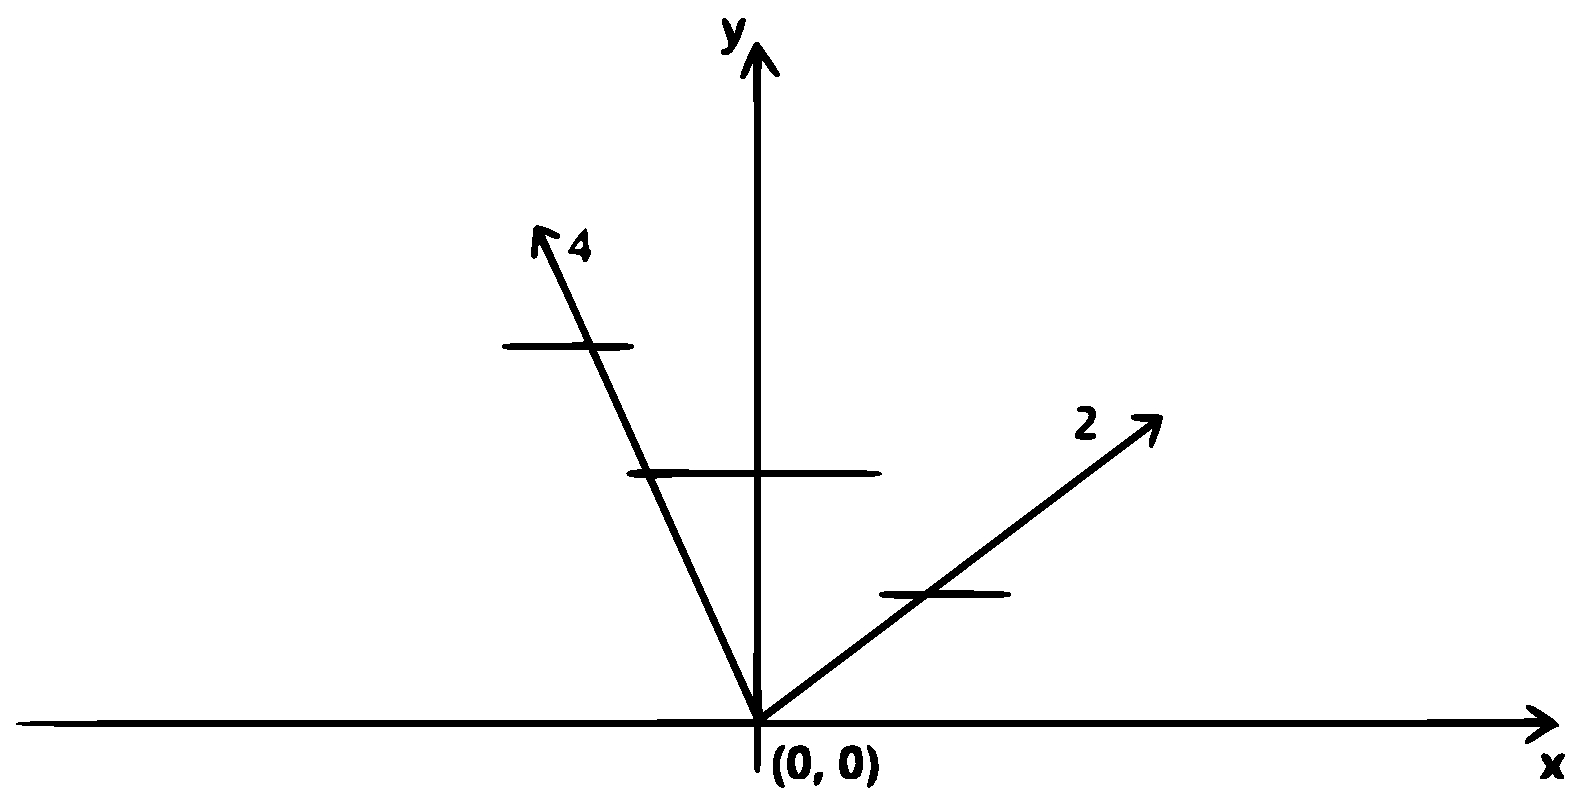
\includegraphics[scale=0.4]{shootgame.eps}}

\end{problem}

